%
%
%
\section{Расчет диаграмм направленности TEM-рупорных антенн}

Из-за большой ширины спектра сигналов, используемых в сверхширокополосных
радиосистемах на СКИ, описание антенны при помощи диаграмм направленности,
используемых обычно в случае узкополосных сигналов, не имеет смысла, так как вид
диаграммы направленности антенны может кардинальным образом образом отличаться
на разных частотах, входящих в спектр СКИ. Поэтому  выглядит целесообразным
использование в этом случае энергетических диаграмм направленности, выражающих
полную энергию, пришедшуюся на то или иное направление за всё время излучения.
Среди пригодных для излучения и приема СКИ сигналов антенн можно выделить
ТЕМ-рупоры с переменным волновым сопротивлением, изменяющимся, как правило,
от~\valu{50}{Ом} в~точке запитки до~$120\pi\,Ом$
у~раскрыва~\cite{bib:Aizenberg1985}. По сути, такая антенна представляет собой
переход с плавно изменяющимся волновым сопротивлением (\emph{плавный переход}).
Однако, форма раскрыва такой рупорной антенны может быть различной. Далее
в~работе рассматриваются два типа антенн: с линейным и экспоненциальным профилем
раскрыва, и исследовалось влияние формы антенны на направленность.

Несмотря на то, что геометрия подобных антенн сложна для аналитических
вычислений, она поддается анализу с помощью численных методов. С помощью метода
FDTD было проведен расчет синтезированных рупоров во временной области, были
построены и проанализированы энергетические диаграммы направленности для
различных сигналов. При этом полное электродинамическое моделирование
выполнялось лишь для одного сигнала, затем по полученному отклику антенны
находились характеристические функции, позволяющие в дальнейшем находить отклик
антенны на сигнал произвольной формы.


\subsection{Вывод уравнений профиля антенны}

Получим выражения, описывающие профиль рупорных антенн с~экспоненциальным
и~линейным раскрывами. Прежде всего введем систему прямоугольных координат.
Пусть антенна расположена симметрично относительно оси~$O_x$ и~главное
направление излучения антенны совпадает с~направлением этой оси, входу антенны
соответствует координата $x=0$. Лепестки антенны расположены симметрично
друг другу относительно плоскости Oxy. Тогда можем записать выражения для
расстояния между лепестками:
\begin{align}
	\label{eq:LinearProfile}
    H(x) &= H_0 + (H_R-H_0)\frac{x}{R}, && \text{(линейный раскрыв)} \\
    \label{eq:ExponentialProfile}
    H(x) &= H_0 \exp
    \left[
        \left(\frac{x}{R}\right)^\alpha\ln\frac{H_R}{H_0}
    \right] && \text{(экспоненциальный раскрыв~\cite{bib:Karshenas2009})}
\end{align}

\noindent
В этих формулах:
\begin{where}
\item $H_0$ --- расстояние между лепестками в~начале раскрыва;
\item $H_R$ --- расстояние между лепестками в~конце раскрыва;
\item $R$ --- длина раскрыва антенны вдоль координаты~$x$.
\end{where}

\noindent
Будем считать антенну длинной линией с~распределенными параметрами, фактически
--- полосковой линией с~переменными шириной и~расстоянием между проводниками.
В~\cite{bib:Aizenberg1985} показано, что уровень отражения входного сигнала
в~длинной линии получается наименьшим, если ее волновое сопротивление изменяется
в~пространстве по~экспоненциальному закону от~входного сопротивления антенны
до~сопротивления нагрузки на~выходе антенны. Итак, волновое сопротивление антенн
(с~обоими рассматриваемыми типами раскрыва) имеет вид:
\begin{equation}
    \label{eq:HornWaveResistance}
    Z(x) = Z_0 \exp
    \left[
        \left(\frac{Z_R}{Z_0}\right)
        \frac{x}{R}
    \right],
\end{equation}
где $Z_0$ --- входное сопротивление антенны, $Z_R$ --- сопротивление нагрузки,
на~которую выполняется согласование.

Теперь воспользуемся известным соотношением для волнового сопротивления
полосковой линии:
\begin{equation}
    \label{eq:MicrostripWaveResistance}
    Z = \frac{H\zeta_0}{B},
\end{equation}
%
\begin{where}
\item $H$ --- расстояние между проводниками линии;
\item $B$ --- ширина проводников;
\item $\zeta_0=120\pi$ --- т.~н. волновое сопротивление вакуума.
\end{where}

\noindent
В~нашей задаче $H$ и~$B$ не~являются постоянными, кроме того, нас интересует
значение ширины лепестка антенны, поэтому выразим его из
формулы~\eqref{eq:MicrostripWaveResistance}:
\begin{equation}
    \label{eq:ProfileWidthFromWaveResistance}
    B(x) = \frac{H(x)\zeta_0}{Z(x)}.
\end{equation}

Подставляя~\eqref{eq:LinearProfile} и~\eqref{eq:ExponentialProfile}
в~\eqref{eq:ProfileWidthFromWaveResistance}, получим после несложных
преобразований окончательные выражения для ширины лепестков антенн:
\begin{align}
    % --
    \label{eq:LinearProfileWidth}
    B(x) &= \frac{\zeta_0}{Z_0}
    \left[ H_0 + (H_R-H_0)\frac{x}{R} \right]
    \exp\left[
        -\frac{x}{R}\ln\frac{Z_R}{Z_0}
    \right] & \text{(линейный)} \\
    % --
    \label{eq:ExponentialProfileWidth}
    B(x) &= \frac{H_0\zeta_0}{Z_0}
    \exp\left[
        \left(\frac{x}{R}\right)^\alpha \ln\frac{H_R}{H_0} -
        \frac{x}{R} \ln\frac{Z_R}{Z_0}
    \right] & \text{(экспоненциальный)}
\end{align}

Это и~есть искомые профили антенн. Графики этих зависимостей при различных
значениях параметра~$Z_R$ изображены на~рис.~\ref{fig:ProfileWidths}
в~разделе~\ref{div:DirectionalPatternExperimentDescription}.


\subsection{Постановка задачи}

Была поставлена задача провести исследование характеристик TEM-рупорных антенн
с~линейным и~экспоненциальным раскрывами. Требуемые выходные сопротивления
антенн:
    \val{150}, \val{200}, \val{250},
    \val{300}, \val{350}, \val{377},
    \val{450}, \valu{500}{Ом}.
(Величина \valu{377}{Ом}, приблизительно равная так называемому волновому
сопротивлению вакуума, взята вместо наиболее близкого к~нему
значению~\valu{400}{Ом} из арифметической прогрессии.) Для каждого значения
выходного сопротивления из этого списка требовалось синтезировать пару рупорных
антенн: с~линейным и~экспоненциальным раскрывами. При этом для всех антенн
неизменными оставались следующие параметры:
\begin{itemize}
\item длина антенны (вдоль оси~$x$):                 $R=\valu{125}{мм}$;
\item расстояние между лепестками в~начальной точке: $H_0=\valu{2}{мм}$;
\item расстояние между лепестками в~конечной точке:  $H_R=\valu{75}{мм}$;
\item параметр~$\alpha$ из
      формулы~\eqref{eq:ExponentialProfile}:         $\alpha=1$;
\item входное сопротивление антенны:                 $Z_0=\valu{50}{Ом}$.
\end{itemize}

\noindent
Требовалось найти отклик антенн и~энергетические диаграммы направленности для
гауссовских униполярных импульсов длительностью~\valu{100}{пс}, \valu{400}{пс}
и~\valu{1000}{пс}.


\subsection{Описание численного эксперимента}
\label{div:DirectionalPatternExperimentDescription}

Для численного эксперимента использовался метод конечных разностей во~временной
области (FDTD) и~его расширения, в~частности, использованы граничные условия
типа идеально согласованного слоя (PML) и~преобразование ближнего поля в~дальнее
(NF-to-FF) при помощи интеграла Кирхгофа. Для этого использовалась программа
\emph{Fdtd3d}, написанная аспирантом кафедры электроники физического факультета
ВГУ Мещеряковым И.\,И. Прежде всего были найдены профили всех антенн. Так,
расстояние между лепестками в~зависимости от~продольной координаты задается
с~помощью формул~\eqref{eq:LinearProfile} и~\eqref{eq:ExponentialProfile}.
Ширина самих лепестков находилась из
соотношения~\eqref{eq:MicrostripWaveResistance} и~задается выведенными там же
формулами~\eqref{eq:LinearProfileWidth} и~\eqref{eq:ExponentialProfileWidth}.
Графики функций~$B(x)$ при различных значениях параметра~$Z_R$ приведены
на~рис.~\ref{fig:ProfileWidths}. Геометрия исследуемых антенн аппроксимировалась
в~счетной области прямоугольными ячейками. Величины шагов дискретизации
по~пространству были выбраны следующими:
\begin{itemize}
\item по оси~$x$: $\Delta{x}=\valu{1.00}{мм}$;
\item по оси~$y$: $\Delta{y}=\valu{1.54}{мм}$;
\item по оси~$z$: $\Delta{z}=\valu{0.50}{мм}$.
\end{itemize}
Шаг дискретизации по~времени рассчитывался автоматически из~условия
Куранта~\eqref{eq:CourantCondition}.

Материал антенны --- медь ($\sigma_E=\valu{5.8E7}{Ом^{-1}}$), а окружающая среда
--- вакуум. В начале раскрыва антенны был установлен ряд точечных резистивных
источников напряжения, на~которые подавался входной сигнал. Для возбуждения
антенны использовался униполярный гауссовский сигнал
длительностью~\valu{100}{пс}. График этого сигнала приведен на
рис.~\ref{fig:DirectionalPatternsSignals}. Для построения диаграммы
направленности вне счетного объема были установлены пробники типа~NF-FF,
распределенные в~плоскостях $O_{xy}$ и~$O_{xz}$ по двум окружностям
радиусом~\valu{30}{м} с~шагом 5~градусов. При этом, в~силу симметрии задачи
и~так как поле позади антенны нас не~интересует, пробники распределялись только
по~четверти длины окружностей. Сама же антенна окружалась прямоугольной
поверхностью, отстоящей от~антенны на 10~шагов дискретизации по~пространству.
По~этой поверхности производилось интегрирование для преобразования ближних
полей в~дальнее. Границы PML отстояли от~поверхности интегрирования еще на
10~шагов дискретизации. Схема эксперимента приведена
на~рис.~\ref{fig:DirectionalPatternExperiment}.


\subsection{Полученные результаты}

После завершения моделирования были получены значения электромагнитных полей
на~пробниках в~каждой временной итерации. Эти значения были были использованы
для построения диаграмм по~методике, описанной
    в~разделе~\ref{div:DirectionalPatternsTheory}
    и~\cite{bib:MescheryakovUnpublishedReport},
а~также для расчета отклика антенны и~её диаграмм направленности при других
входных сигналах при помощи импульсных характеристик. Для упрощения анализа
проведем сравнение только двух антенн: с~выходным волновым сопротивлением
\valu{377}{Ом} и~разными типами раскрыва. В~дальнейшем все графики относятся
именно к~этим антеннам.

Графики тока и~напряжения, полученные на~выходе антенн при моделировании
(на вход антенны подавался сигнал длительностью \valu{100}{нс}) приведены
    на~рис.~\ref{fig:ReplyVoltages377}
    и~\ref{fig:ReplyCurrents377}.
Полученные диаграммы направленности приведены:
\begin{itemize}
\item для сигнала длительностью~\valu{100}{пс} (исходного) ---
      на~рис.~\ref{fig:DirectionalPattern100ps};
\item для сигнала длительностью~\valu{400}{пс} ---
      на~рис.~\ref{fig:DirectionalPattern400ps};
\item для сигнала длительностью~\valu{1000}{пс} ---
      на~рис.~\ref{fig:DirectionalPattern1000ps}.
\end{itemize}


\subsection{Анализ полученных результатов}

Обратимся к~диаграммам направленности. Можно видеть, что антенна
с~экспоненциальным профилем раскрыва обладает значительно более узкой диаграммой
направленности в~вертикальной плоскости и~в~то же время более широкой диаграммой
в~горизонтальной плоскости.

\paragraph{Излучение сигнала длительностью~100~пс.\\}
Пространственная длительность данного сигнала меньше длины антенны. В~этом
случае антенна с~экспоненциальным раскрывом обладает значительно лучшей
направленностью как по углу~$\phi$, так и~по углу~$\theta$.

\paragraph{Излучение сигнала длительностью~400~пс.\\}
Пространственная длительность данного сигнала примерно соответствует длине
антенны. В~этом случае направленность антенны с~экспоненциальным профилем
по~углу~$\theta$ по-прежнему значительно лучше, чем антенны с~линейным
раскрывом. В~то же время направленность по углу~$\phi$ экспоненциальной антенны
несколько хуже, чем линейной.

\paragraph{Излучение сигнала длительностью~1000~пс.\\}
Пространственная длительность данного сигнала значительно больше длины антенны.
Направленность антенны с~экспоненциальным профилем как по~$\phi$, так
и~по~$\theta$ значительно ухудшилась по~сравнению с~антенной с~линейным
профилем.

Из сказанного заключим, что применение антенн с~экспоненциальным раскрывом
вместо антенн с~линейным раскрывом более собразно при использовании сигналов
с~пространственной длительностью, меньшей длины антенны.

%% --
\begin{figure}
\label{fig:DirectionalPatternExperiment}
\centering
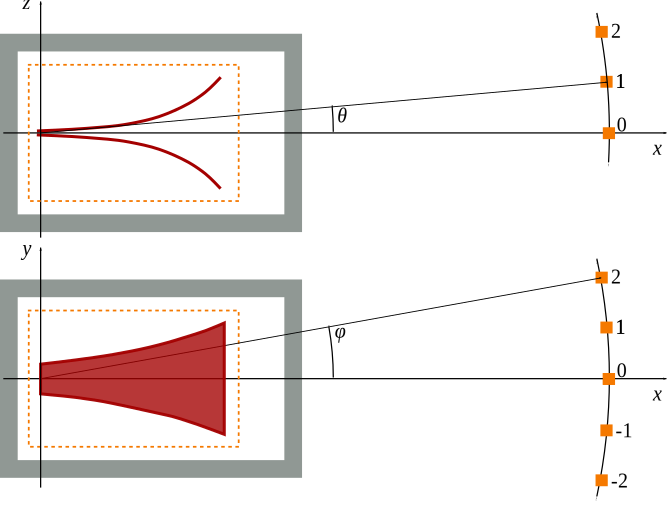
\includegraphics[width=0.7\textwidth]{graphics/directional-patterns-experiment-scheme}
\caption{
    Схема эксперимента, вид в~профиль (вверху), вид сверху (внизу).
    Прямоугольниками обозначены пробники для преобразования ближнего поля
    в~дальнее, пунктирная рамка обозначает поверхность интегрирования для
    интеграла Кирхгофа. Угловое расстояние между пробниками составляет
    5~градусов.}
\end{figure}

%% --
\begin{figure}
\label{fig:DirectionalPatternsSignals}
\centering
\includegraphics[width=0.7\textwidth]{graphics/directional-patterns-signals}
\caption{
    Входные сигналы антенны --- униполярные гауссовские импульсы различной
    длительности. Красная линия изображает сигнал длительностью~\valu{100}{пс},
    оранжевая --- длительностью~\valu{400}{пс},
    желтая --- длительностью~\valu{1000}{пс}.
    Длительность импульса определялась по~уровню 1/10.}
\end{figure}

%% --
\begin{figure}
\label{fig:ReplyVoltages377}
\centering
\includegraphics[width=0.7\textwidth]{graphics/directional-patterns-reply-linear-U}
\includegraphics[width=0.7\textwidth]{graphics/directional-patterns-reply-exponential-U}
\caption{
    Напряжения на~выходе антенн с~линейным (вверху) и~экспоненциальным (внизу)
    профилями, синтезированными для выходного сопротивления~\valu{377}{Ом}.}
\end{figure}

%% --
\begin{figure}
\label{fig:ReplyCurrents377}
\centering
\includegraphics[width=0.7\textwidth]{graphics/directional-patterns-reply-linear-I}
\includegraphics[width=0.7\textwidth]{graphics/directional-patterns-reply-exponential-I}
\caption{
    Токи на~выходе антенн с~линейным (вверху) и~экспоненциальным (внизу)
    профилями, синтезированными для выходного сопротивления~\valu{377}{Ом}.}
\end{figure}

%% --
\begin{figure}
\label{fig:ProfileWidths}
\centering
\includegraphics[width=0.7\textwidth]{graphics/directional-patterns-profile-widths}
\caption{
    Зависимость ширины лепестков исследуемых антенн от~значения продольной
    координаты при различных значениях параметра~$Z_R$. Сплошными линиями
    обозначены профили антенн с~линейным раскрывом, пунктирными --- профили
    антенны с~экспоненциальными раскрывами. Видно, что конечные точки профилей
    с~одинаковым волновым сопротивлением совпадают, как и~должно быть согласно
    теории. Подписи на~графике относятся к~паре антенн с~данной конечной точкой.}
\end{figure}

% ---
\begin{figure}
\label{fig:DirectionalPattern100ps}
\centering
\includegraphics[width=0.7\textwidth]{graphics/directional-patterns-100ps-phi}
\includegraphics[width=0.7\textwidth]{graphics/directional-patterns-100ps-theta}

\caption{
    Сравнение энергетических диаграмм направленности в~горизонтальной (вверху)
    и~вертикальной плоскостях~(внизу) для двух антенн, синтезированных для
    выходного сопротивления~\valu{377}{Ом}, при возбуждении сигналом
    длительностью~\valu{100}{пс}. Красным цветом изображены диаграммы
    направленности антенны с~линейным раскрывом, оранжевым ---
    с~экспоненциальным.}
\end{figure}

% ---
\begin{figure}
\label{fig:DirectionalPattern400ps}
\centering
\includegraphics[width=0.7\textwidth]{graphics/directional-patterns-400ps-phi}
\includegraphics[width=0.7\textwidth]{graphics/directional-patterns-400ps-theta}

\caption{
    Сравнение энергетических диаграмм направленности в~горизонтальной (вверху)
    и~вертикальной плоскостях~(внизу) для двух антенн, синтезированных для
    выходного сопротивления~\valu{377}{Ом}, при возбуждении сигналом
    длительностью~\valu{400}{пс}. Красным цветом изображены диаграммы
    направленности антенны с~линейным раскрывом, оранжевым ---
    с~экспоненциальным.}
\end{figure}

% ---
\begin{figure}
\label{fig:DirectionalPattern1000ps}
\centering
\includegraphics[width=0.7\textwidth]{graphics/directional-patterns-1000ps-phi}
\includegraphics[width=0.7\textwidth]{graphics/directional-patterns-1000ps-theta}

\caption{
    Сравнение энергетических диаграмм направленности в~горизонтальной (вверху)
    и~вертикальной плоскостях~(внизу) для двух антенн, синтезированных для
    выходного сопротивления~\valu{377}{Ом}, при возбуждении сигналом
    длительностью~\valu{1000}{пс}. Красным цветом изображены диаграммы
    направленности антенны с~линейным раскрывом, оранжевым ---
    с~экспоненциальным.}
\end{figure}
